% #####################################################################
% #####################################################################
% ##                                                                 ##
% ##                             Lizenz:                             ##
% ##                         CC BY-NC-SA 3.0                         ##
% ##      http://creativecommons.org/licenses/by-nc-sa/3.0/de/       ##
% ##                                                                 ##
% #####################################################################
% ##   Diese Datei kann beliebig verändert werden, solange darauf    ##
% ##     hingewiesen wird, dass dieses Dokument ursprünglich von     ##
% ##                                                                 ##
% ##                        www.ei-studium.de                        ##
% ##                                                                 ##
% ##                             stammt.                             ##
% ## Dies gilt insbesondere auch für alle daraus erstellten Dateien. ##
% ##    Des Weiteren muss die Weitergabe dieser Dateien unter der    ##
% ##                    gleichen Lizenz erfolgen.                    ##
% #####################################################################
% #####################################################################
\documentclass[a4paper,twocolumn,10pt]{article}
\usepackage[utf8]{inputenc}
\usepackage[ngerman]{babel}
\usepackage[top=2.0cm,bottom=1.5cm,left=1.0cm,right=1.0cm]{geometry}
\usepackage{enumitem}
\usepackage{graphicx}
\usepackage{amsfonts}
\usepackage{amsmath}
\usepackage{sectsty}
\usepackage{colortbl}
\usepackage{cancel}
\usepackage{listings}
\usepackage{color}
\usepackage{epstopdf}
\usepackage{fancyhdr}
\usepackage[european]{circuitikz}
\usepackage{adjustbox}
\usepackage{subfig}
\usepackage{pgfplots}
\pgfplotsset{width=8cm,compat=1.9} 
\setlength{\intextsep}{0pt}

\setlist{itemsep=.01mm}
\setenumerate{label=\emph{\arabic*})}
\setlength{\columnsep}{1cm}
\parindent 0mm

\partfont{\huge}
\sectionfont{\Large \sc\bf}
\subsectionfont{\normalsize}
\subsubsectionfont{\small\textit}

\pagestyle{fancy}
\lhead[\leftmark]{Schaltungstechnik 1}
\chead[\leftmark]{TEAM INFORMATIK (Vorlage von www.ei-studium.de)}
\rhead[\leftmark]{Erstelldatum: \today}
\lfoot[\leftmark]{Keine Garantie auf Vollständigkeit und Richtigkeit!}
\cfoot[\leftmark]{}
\rfoot[\leftmark]{\textbf{Seite \thepage}}
\renewcommand{\headrulewidth}{0.5pt}
\renewcommand{\footrulewidth}{0.5pt}

\newcommand*\kreis[1]{\unitlength1ex\begin{picture}(2.5,2.5)%
\put(0.75,0.75){\circle{3}}\put(0.7,0.7){\makebox(0,0){#1}}\end{picture}}

\begin{document}

\part*{Schaltungstechnik 1}

\section*{Kirchhoff-Gesetze}
\subsection*{Anwendbarkeit}
Konzentriertheitshypothese muss erfüllt sein:\\
$d<<\lambda = \frac{c}{f}$\\
d: Größe der Schaltung\\
$\lambda$: Wellenlänge

\subsection*{Netzwerktheorie}
Zweige: Anzahl Kanten\\
Knoten: Anzahl Spannungsknoten (inklusive Masse wenn existiert).\\
Richtung Kantenpfeil $\equiv$ Richtung Kantenstrom und Kantenspannung.\\
Graph besteht aus Baum und Verbindungskanten.

\subsection*{Knoteninzidenzmatrix}
Matrix $A\in \{-1, 0, 1\}^{(n-1)\times(b)}$\\
Eintrag $a_{\alpha\beta}=\begin{cases}+1,&\text{Outgoing, Zweig }\beta\leftarrow\text{Knoten }\alpha\\-1,&\text{Incoming, Zweig }\beta\rightarrow\text{Knoten }\alpha\\\pm0,&\text{Kein Zweig }\beta\leftrightarrow\text{Knoten }\alpha\end{cases}$\\
Beinhaltet nicht den Bezugsknoten (da linear abhängig).

\subsection{KVL Matrix}
Matrix $B\in \{-1, 0, 1\}^{b\times b-(n-1)}$\\
Eintrag $b_{\alpha\beta}=\begin{cases}+1,&\text{Zweig in Richtung Masche}\\-1,&\text{Zweig entgegen Masche}\\\pm0,&\text{Kein Zweig in Masche}\end{cases}$\\

\subsection*{Knotenregel (KCL)}
Für jeden Knoten gilt:\\
Die Summe aller Ströme ist Null.\\
$\sum\limits_{Knoten}^{} i_j(t)=0$\\\\
(herausfließende Ströme positiv)\\\\
Anzahl linear unabhängiger Knotengleichungen: $\textbf{(n-1)}$\\
n: Anzahl der Knoten\\\\
KCL in Matrixform:\\
Nullraumdarstellung: $\textbf{A}\cdot \underline{i}=\underline{0}$\\
Mit Knoteninzidenzmatrix \textbf{A}

\subsection*{Maschenregel (KVL)}
Für jede Masche gilt:\\
Die Summe der Teilspannungen ist Null.\\
$\sum\limits_{Umlauf}^{} u_j(t)=0$\\\\
(Spannungen in Umlaufrichtung positiv)\\\\
Anzahl linear unabhängiger Schleifengleichungen: $\textbf{b-(n-1)}$\\
b: Anzahl der Zweige\\
n: Anzahl der Knoten\\\\
KVL in Matrixform:\\
Nullraumdarstellung: $\textbf{B}\underline{u}=0$\\
$\underline{u}$ ist Spannungen der Kanten\\$\underline{u}-\textbf{A}^T\cdot \underline{u_k}=\underline{0}$\\
Bildraumdarstellung: $\underline{u}=\textbf{A}^T\cdot\underline{u_k}$\\
$(\textbf{M}=\textbf{A}^T)$ Mit Inzidenzmatrix $\textbf{A}$

\section*{Resistive Eintore}
\subsection*{Darstellungsformen}
\begin{tabular}{ll}
Implizit: & $f_F(u,i)=0$\\
Explizit: & $u=r(i), i=g(u)$\\
Parametrisiert: & $u=u(\lambda), i=i(\lambda)$
\end{tabular}

\subsection*{Eigenschaften}
\begin{tabular}{ll}
\textbf{$F$ ist...} & \textbf{Kennlinie von $F$...}\\
- stromgesteuert & $\exists$ Darstellung $u=r(i)$\\
- spannungsgesteuert & $\exists$ Darstellung $i=g(u)$\\
- ungepolt & ... ist punktsymmetrisch zu (0/0)\\
- passiv & ... verläuft nur im I. oder III. Quadr.\\
- aktiv & ... ist nicht passiv\\
- verlustlos & ... liegt nur auf den Achsen\\
- quellenfrei & ... geht durch den Ursprung\\
- streng linear & ... ist Ursprungsgerade, Ursprung\\
 & \;\;\;\;oder ganze u-i-Ebene\\
- linear & ... ist eine beliebige Gerade\\
- stückweise linear & ... besteht aus Geradenstücken
\end{tabular}

\subsection*{Umpolung}
Punktspiegelung der Kennline am Ursprung\\
$(u,i)\in F \Leftrightarrow (-u,-i)\in \overline{F}$

\subsection*{Dualität}
Für $R_d=1 \Omega$: Spiegelung an der Winkelhalbierenden.\\
$(u,i)\in F \Leftrightarrow (R_di,\frac{u}{R_d})\in F^d$

\subsection*{Widerstände}
\begin{tabular}{lll}
$u=R\cdot i$ & $R=\frac{1}{G}$ & $R_1||R_2 = \frac{R_1\cdot R_2}{R_1+R_2}$ (Parallel)
\end{tabular}\\\\
\begin{tabular}{ll}
Reihenschaltung: & $R_{gesamt}=R_1+...+R_i$\\
Parallelschaltung: & $\frac{1}{R_{gesamt}}=\frac{1}{R_1}+...+\frac{1}{R_i}$ 
\end{tabular}

\subsection*{Leitwerte}
\begin{tabular}{lll}
$i=G\cdot u$ & $G=\frac{1}{R}$ & $G_1||G_2 = \frac{G_1\cdot G_2}{G_1+G_2}$ (Seriell)\\ & & \\
\end{tabular}
\begin{tabular}{ll}
Reihenschaltung: & $\frac{1}{G_{gesamt}}=\frac{1}{G_1}+...+\frac{1}{G_i}$\\
Parallelschaltung: & $G_{gesamt}=G_1+...+G_i$
\end{tabular}

\subsection*{Spannungsteiler / Stromteiler}

\begin{minipage}[t]{0.23\textwidth}
\centering
Spannungsteiler\\
\vspace{0.3 cm}
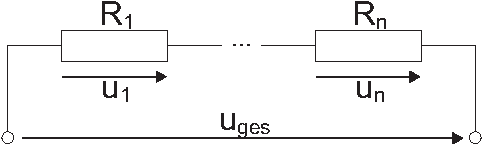
\includegraphics[width=0.8\textwidth]{img/Spannungsteiler}\\
\vspace{0.5 cm}
$u_i=u_{ges}\cdot \frac{R_i}{R_{ges}}=u_{ges}\cdot \frac{G_{ges}}{G_i}$
$R_{ges}=R_1+...+R_n$
$G_{1+2}=\frac{G_1\cdot G_2}{G_1+G_2}$
\end{minipage}
\hfill
\begin{minipage}[t]{0.23\textwidth}
\centering
Stromteiler\\
\vspace{0.3 cm}
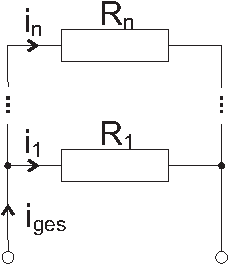
\includegraphics[width=0.5\textwidth]{img/Stromteiler}\\
\vspace{0.5 cm}
$i_i=i_{ges}\cdot \frac{R_{ges}}{R_i}=i_{ges}\cdot \frac{G_i}{G_{ges}}$
$G_{ges}=G_1+...+G_n$
$R_{1+2}=\frac{R_1\cdot R_2}{R_1+R_2}$
\end{minipage}
\\
\begin{minipage}{0.20\textwidth}
	$u_{ges}=R_{ges}i_{ges}$\\
	$R_{ges}=R_2+\frac{R_2R_3}{R_2+R_3}$\\\\
	$u_{R1}=\frac{1}{1+\frac{R_2 R_3}{R_1(R_2 + R_3)}}u_{ges}$\\
	$u_{R2}=\frac{1}{1+\frac{R_1(R_2+R_3)}{R_2R_3}}u_{ges}$\\
	$u_{R3}=u_{R2}$
	\\\\
	$i_{R1}=i_{ges}$\\
	$i_{R2}=\frac{R_3}{(R_2+R_3)}i_{ges}$\\
	$i_{R3}=\frac{R_2}{(R_2+R_3)}i_{ges}$
\end{minipage}
\begin{minipage}{0.28\textwidth}
	\begin{circuitikz}
		\draw(0,4)
		to[short, i=$i_{ges}$, o-] (2,4);
		\draw(0,0)
		to[short, o-*] (2,0)
		to[R=$R_2$,v=$U_{R2}$, -*] (2,2)
		to[R=$R_1$,v=$U_{R1}$] (2,4);
		\draw(2,0)
		to[short] (4,0)
		to[R=$R_3$,v=$U_{R3}$] (4,2);
		\draw(2,2)
		to[short,i=$i_{R3}$] (4,2);
		\draw(0,4)
		to[open,v>=$u_{ges}$] (0,0);
	\end{circuitikz}
\end{minipage}


\subsection*{Quellwandlung linearer Quellen}
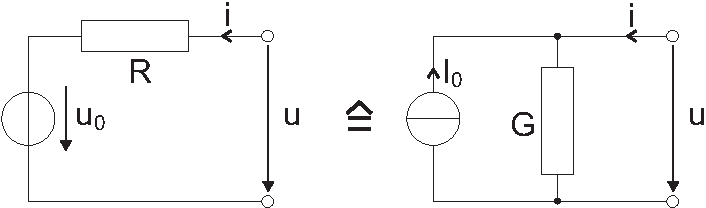
\includegraphics[width=0.45\textwidth]{img/Quellwandlung}\\\\
\textbf{Wichtig: Pfeilrichtung $I_0$} \\
Für jede lineare Quelle gilt:\\
$u=R_i\cdot i+U_0$ bzw. $i=G_i\cdot u-I_0$

\subsection*{Kennlinienbestimmung von verschalteten Bauteilen}
\subsubsection*{Parallel}
Die Spannung ist an jedem Bauteil gleich. Die Ströme werden nach der Knotenregel addiert.\\
Grafisch: Kennlinien entlang der i-Achse addieren.\\
\begin{figure}[h]
	\centering
	\minipage{0.1\textwidth}
			\begin{adjustbox} {max height = 100pt}
			\begin{circuitikz}
				\draw (0,4)
				to[V,v=$U_{q1}$] (2,4) % The voltage source
				to[short] (2,0)
				to[R=$R_L$] (0,0)
				to[short] (0,4);
				\draw (0,2)
				to[V,v=$U_{q2}$] (2,2);
			\end{circuitikz}
	\end{adjustbox}

	\endminipage
			$\Rightarrow$
	\minipage{0.2\textwidth}
			\begin{adjustbox} {max width = \textwidth, max height=100pt}
				\begin{tikzpicture}
				\begin{axis}[
				axis lines = center,
				xlabel = $u$,
				ylabel = {$i$},
				ymin=0,
				ymax=2.5,
				]
				%Below the red parabola is defined
				\addplot [
				domain=-3:3, 
				samples=100, 
				color=red,
				]
				{1.5};
				\addlegendentry{$\mathcal{F}_1$}
				%Here the blue parabloa is defined
				\addplot [
				domain=-3:3, 
				samples=100, 
				color=blue,
				]
				{0.5};
				\addlegendentry{$\mathcal{F}_2$}
				
				\addplot [
				domain=-3:3, 
				samples=100, 
				color=green,
				]
				{2.0};
				\addlegendentry{$\mathcal{F}_{1+2}$}
				
				
				\end{axis}
				\end{tikzpicture}
			\end{adjustbox}
	\endminipage

\end{figure}

\subsubsection*{Seriell}
Der Strom ist in jedem Bauteil gleich. Die Spannungen werden nach der Maschenregel addiert.\\
Grafisch: Kennlinien entlang der u-Achse addieren.

\begin{figure}[h]
	\centering
	\minipage{0.1\textwidth}
	\begin{adjustbox} {max height = 100pt}
		\begin{circuitikz}
			\draw (0,4)
			to[I,i=$I_{q1}$] (2,4) % The voltage source
			to[short] (2,0)
			to[R=$R_L$] (0,0)
			to[short] (0,4);
			\draw (0,2)
			to[I,i=$I_{q2}$] (2,2);
		\end{circuitikz}
	\end{adjustbox}
	
	\endminipage
	$\Rightarrow$
	\minipage{0.2\textwidth}
	\begin{adjustbox} {max width = \textwidth, max height=100pt}
		\begin{tikzpicture}
		\begin{axis}[
		axis lines = center,
		xlabel = $u$,
		ylabel = {$i$},
		ymin=0,
		ymax=2.5,
		xmin=0,
		xmax=2.5
		]
		%Below the red parabola is defined
		\addplot +[mark=none] coordinates {(0.5, 0) (0.5, 3)};
		\addlegendentry{$\mathcal{F}_1$}
		%Here the blue parabloa is defined
		\addplot +[mark=none, color=red] coordinates {(1.5, 0) (1.5, 3)};
		\addlegendentry{$\mathcal{F}_2$}
		\addplot +[mark=none, color=green] coordinates {(2, 0) (2, 3)};		\addlegendentry{$\mathcal{F}_{\setlength{\intextsep}{0pt}1+2}$}
		
		
		\end{axis}
		\end{tikzpicture}
	\end{adjustbox}
	\endminipage
	
\end{figure}

\subsection*{Arbeitspunktbestimmung}
\begin{tabular}{ll}
$Q$: & Quelleneintor\\
$Q^x$: & Quelleneintor gespiegelt an der u-Achse\\
$F$: & Lasteintor
\end{tabular}
\begin{minipage}[b]{0.23\textwidth}
\centering
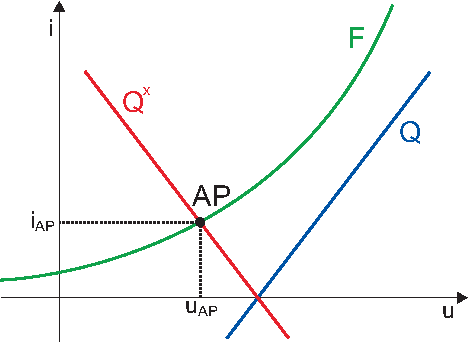
\includegraphics[width=0.8\textwidth]{img/Arbeitspunkt}\\
\end{minipage}
\hfill
\begin{minipage}[b]{0.23\textwidth}
Rechnerisch: $i_Q=-i_F$\\\\
Graphisch: $AP=F\cap Q^x$
\end{minipage}

\subsection*{Linearisierung im Arbeitspunkt}
z.B. Leitwertsbeschreibung:\\\\
$\Delta i_F=\left.\frac{\partial i_F}{\partial u_F} \right|_{AP}\cdot \Delta u_F$\\\\
$(i_F=I_{AP}+\Delta i_F;\;\;\;u_F=U_{AP}+\Delta u_F)$\\\\
$i_{F,lin}=\left.\frac{\partial i_F}{\partial u_F} \right|_{AP}\cdot (u_F-U_{AP})+I_{AP}$\\\\
$i_{F,lin}=\underbrace{\left.\frac{\partial i_F}{\partial u_F} \right|_{AP}}_{g}\cdot u_F-\underbrace{\left.\frac{\partial i_F}{\partial u_F} \right|_{AP}\cdot U_{AP}+I_{AP}}_{I_{0,AP}}$

\subsection*{Ersatzschaltbilder}
Zuerst alle Bauteile im Arbeitspunkt linearisieren. Erhalte $u_1=U+\Delta u$\\
%\subsubsection*{Groß-/Kleinsignal}
\textbf{Großsignal:} Alle Wechselquellen weglassen. $u_1=U$\\
\textbf{Kleinsignal:} Alle Konstantquellen weglassen. $U_1=\Delta u$ 
\subsubsection*{Ersetzen von Quellen}
\begin{figure}[h]
	\centering
	\begin{minipage}{0.1\textwidth}
		\begin{circuitikz}
			\draw(0,2)
			to[V,v=$U_1$] (0,0);
		\end{circuitikz}
	\end{minipage}
	$\Rightarrow$
	\begin{minipage}{0.03\textwidth}
		\begin{circuitikz}
			\draw(0,2)
			to[short] (0,0);
		\end{circuitikz}
	\end{minipage}
	\&  
	\begin{minipage}{0.1\textwidth}
		\begin{circuitikz}
			\draw(0,2)
			to[I,i=$I_1$] (0,0);
		\end{circuitikz}
	\end{minipage}
	$\Rightarrow$
	\begin{minipage}{0.03\textwidth}
		\begin{circuitikz}
			\draw(0,2)
			to[short] (0,1.3);
			\draw(0,0)
			to[short] (0,0.7);
		\end{circuitikz}
	\end{minipage}
\end{figure}

\subsection*{Bauelemente}
\subsubsection*{Nullator}
\begin{minipage}[b]{0.26\textwidth}
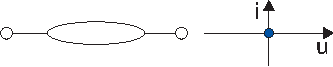
\includegraphics[width=0.95\textwidth]{img/Nullator}
\end{minipage}
\hfill
\begin{minipage}[b]{0.2\textwidth}
$u=0$\\
$i=0$
\end{minipage}
Strom/spannungsgesteuert, ungepolt, passiv, verlustlos, quellenfrei, streng linear. Dual zu Nullator.

\subsubsection*{Norator}
\begin{minipage}[b]{0.26\textwidth}
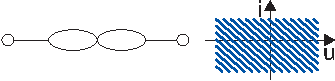
\includegraphics[width=0.95\textwidth]{img/Norator}
\end{minipage}
\hfill
\begin{minipage}[b]{0.2\textwidth}
$u=$ beliebig\\
$i=$ beliebig
\end{minipage}
Ungepolt, aktiv, quellenfrei, streng linear. Dual zu Norator.

\subsubsection*{Leerlauf}
\begin{minipage}[b]{0.26\textwidth}
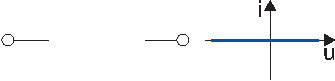
\includegraphics[width=0.95\textwidth]{img/Leerlauf}
\end{minipage}
\hfill
\begin{minipage}[b]{0.2\textwidth}
$u=$ beliebig\\
$i=0$
\end{minipage}
Spannungsgesteuert, ungepolt, passiv, verlustlos, quellenfrei, streng linear. Dual zu Kurzschluss.

\subsubsection*{Kurzschluss}
\begin{minipage}[b]{0.26\textwidth}
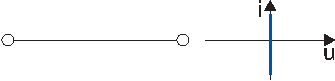
\includegraphics[width=0.95\textwidth]{img/Kurzschluss}
\end{minipage}
\hfill
\begin{minipage}[b]{0.2\textwidth}
$u=0$\\
$i=$ beliebig
\end{minipage}
Stromgesteuert, ungepolt, passiv, verlustlos, quellenfrei, streng linear. Dual zu Leerlauf.

\subsubsection*{Ohmscher Widerstand}
\begin{minipage}[b]{0.26\textwidth}
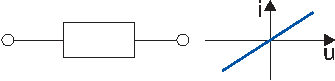
\includegraphics[width=0.95\textwidth]{img/Widerstand}
\end{minipage}
\hfill
\begin{minipage}[b]{0.2\textwidth}
$u=R\cdot i$\\
$i=G\cdot u$
\end{minipage}
Spannungs-/Stromgesteuert ($R>0$/$G>0$), ungepolt, passiv für $R\ge 0$, aktiv für $R<0$, quellenfrei, streng linear. Dual zu Widerstand mit $R_2=\frac{1}{R_1}$.

\subsubsection*{Ideale Stromquelle}
\begin{minipage}[b]{0.26\textwidth}
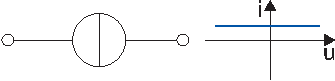
\includegraphics[width=0.95\textwidth]{img/Stromquelle}
\end{minipage}
\hfill
\begin{minipage}[b]{0.2\textwidth}
$u=$ beliebig\\
$i=I_0$
\end{minipage}
Für $I>0$: Spannungsgesteuert, gepolt, aktiv, nicht verlustlos, nicht quellenfrei, linear. Dual zu Spannungsquelle.

\subsubsection*{Ideale Spannungsquelle}
\begin{minipage}[b]{0.26\textwidth}
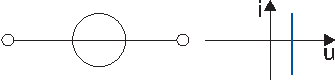
\includegraphics[width=0.95\textwidth]{img/Spannungsquelle}
\end{minipage}
\hfill
\begin{minipage}[b]{0.2\textwidth}
$u=U_0$\\
$i=$ beliebig
\end{minipage}
Für $U>0$: Stromgesteuert, gepolt, aktiv, nicht verlustlos, nicht quellenfrei, linear. Dual zu Stromquelle.

\subsubsection*{Ideale Diode}
\begin{minipage}[b]{0.26\textwidth}
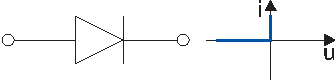
\includegraphics[width=0.95\textwidth]{img/IdealeDiode}
\end{minipage}
\hfill
\begin{minipage}[b]{0.2\textwidth}
$u=0$ für $i>0$\\
$i=0$ für $u<0$
\end{minipage}
Nicht Strom/Spannungsgesteuert, gepolt, passiv, quellenfrei, stückweise linear. Dual zu umgepoltem selbst.

\subsubsection*{Reale Diode}
\begin{minipage}[b]{0.26\textwidth}
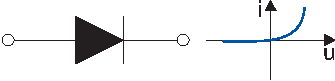
\includegraphics[width=0.95\textwidth]{img/RealeDiode}
\end{minipage}
\hfill
\begin{minipage}[b]{0.2\textwidth}
$u=U_T\cdot ln(\frac{i}{I_S}+1)$\\
$i=I_S(e^{\frac{u}{U_T}}-1)$
\end{minipage}
Spannungs/Stromgesteuert, gepolt, passiv, quellenfrei, nicht linear.

\subsubsection*{Photodiode}
\begin{minipage}[b]{0.24\textwidth}
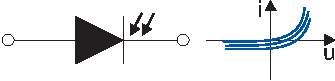
\includegraphics[width=\textwidth]{img/Photodiode}
\end{minipage}
\hfill
\begin{minipage}[b]{0.22\textwidth}
$u(t)=U_T\cdot ln(\frac{i(t)+i_L(t)}{I_S}+1)$\\
$i(t)=I_S(e^{\frac{u(t)}{U_T}}-1)-i_L(t)$
\end{minipage}
Nicht Strom/Spannungsgesteuert, gepolt, aktiv, nicht linear.

\subsubsection*{Zenerdiode}
\begin{minipage}[b]{0.26\textwidth}
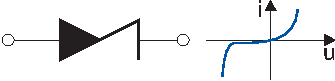
\includegraphics[width=0.95\textwidth]{img/Z-Diode}
\end{minipage}
\hfill
\begin{minipage}[b]{0.2\textwidth}
leitet bei $u<U_Z$
\end{minipage}
Strom/Spannungsgesteuert, gepolt, passiv, quellenfrei, nicht linear.

\subsubsection*{Tunneldiode}
\begin{minipage}[b]{0.26\textwidth}
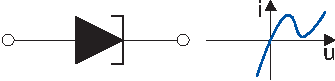
\includegraphics[width=0.95\textwidth]{img/Tunneldiode}
\end{minipage}
\\
Spannungsgesteuert, gepolt, passiv, quellenfrei, nicht linear.

\subsubsection*{Konkaver Widerstand}
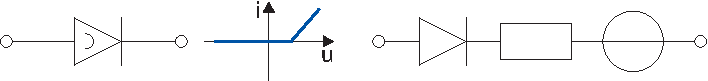
\includegraphics[width=0.48\textwidth]{img/Rkonkav}\\\\
$i=0$ für $u\leq U_0$\\
$i=G\cdot (u-U_0)$ für $u\geq U_0$\\
Spannungsgesteuert, gepolt, passiv, quellenfrei ($U_0\ge 0$), stückweise linear. Dual zu konvexem Widerstand.

\subsubsection*{Konvexer Widerstand}
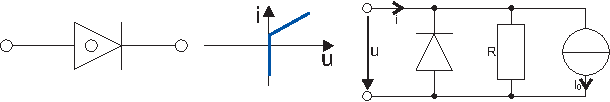
\includegraphics[width=0.48\textwidth]{img/Rkonvex}\\\\
$u=0$ für $i\leq I_0$\\
$u=R\cdot (i-I_0)$ für $i\geq I_0$\\
Stromgesteuert, gepolt, passiv, quellenfrei ($I_0\geq 0$), stückweise linear.

\subsubsection*{Lineare Quellen}
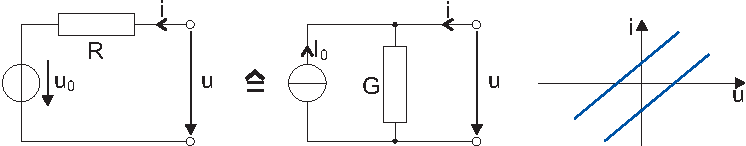
\includegraphics[width=0.48\textwidth]{img/lineareQuellen}\\\\
$U_0=I_0\cdot R;\;\;\;I_0=U_0\cdot G$
Spannungs/Stromgesteuert ($R>0$/$G>0$), gepolt, aktiv ($I_0>0 \Leftrightarrow U_0>0$), linear.

\section*{Resistive Zweitore}
\subsection*{Darstellungsformen}
\subsubsection*{Implizit}
\begin{tabular}{ll}
$\underbrace{\begin{bmatrix}\textbf{M} & \textbf{N}\end{bmatrix}\cdot \left.\begin{matrix}\underline{u}\\\underline{i}\end{matrix}\right]=\underline{0}}_{Kern\begin{bmatrix}\textbf{M} & \textbf{N}\end{bmatrix}}$ & quellenfrei\\\\
$F=Kern\begin{bmatrix}\textbf{M} & \textbf{N}\end{bmatrix}+\left.\begin{matrix}\underline{u_0}\\\underline{i_0}\end{matrix}\right]$ & nicht quellenfrei
\end{tabular}\\
Explizit $\Rightarrow$ Implizit: $i=Gu\Rightarrow 0=Gu-1\Rightarrow [M N]=[G -1]$
\subsubsection*{Explizit}
Größe mit konstantem Nullwert (KS, LL, Nullator) kann keine Steuergröße sein. Größe mit beliebigem Wert (Norator) kann nicht gesteuert werden.
\begin{tabular}{ll}
	$\left.\begin{matrix}i_1\\i_2\end{matrix}\right] =\textbf{G}\cdot \left.\begin{matrix}u_1\\u_2\end{matrix}\right]=\left.\begin{matrix}g_{11}u_1+g_{12}u_2\\g_{21}u_1+g_{22}u_2\end{matrix}\right]$ &
	Leitwertsbeschr.\\\\
	$\left.\begin{matrix}u_1\\u_2\end{matrix}\right] =\textbf{R}\cdot \left.\begin{matrix}i_1\\i_2\end{matrix}\right]=\left.\begin{matrix}r_{11}i_1+r_{12}i_2\\r_{21}i_1+r_{22}i_2\end{matrix}\right]$ &
	Widerstandsbeschr.\\\\
	$\left.\begin{matrix}u_1\\i_2\end{matrix}\right] =\textbf{H}\cdot \left.\begin{matrix}i_1\\u_2\end{matrix}\right]=\left.\begin{matrix}h_{11}i_1+h_{12}u_2\\h_{21}i_1+h_{22}u_2\end{matrix}\right]$ &
	hybride Beschr.\\\\
	$\left.\begin{matrix}i_1\\u_2\end{matrix}\right] =\textbf{H'}\cdot \left.\begin{matrix}u_1\\i_2\end{matrix}\right]=\left.\begin{matrix}h'_{11}u_1+h'_{12}i_2\\h'_{21}u_1+h'_{22}i_2\end{matrix}\right]$ &
	inverse hybride Beschr.\\\\
	$\left.\begin{matrix}u_1\\i_1\end{matrix}\right] =\textbf{A}\cdot \left.\begin{matrix}u_2\\-i_2\end{matrix}\right]=\left.\begin{matrix}a_{11}u_2-a_{12}i_2\\a_{21}u_2-a_{22}i_2\end{matrix}\right]$ &
	Kettenbeschr.\\\\
	$\left.\begin{matrix}u_2\\i_2\end{matrix}\right] =\textbf{A'}\cdot \left.\begin{matrix}u_1\\-i_1\end{matrix}\right]=\left.\begin{matrix}a'_{11}u_1-a'_{12}i_1\\a'_{21}u_1-a'_{22}i_1\end{matrix}\right]$ &
	inverse Kettenbeschr.
\end{tabular}

\subsubsection*{Parametrisiert}
\begin{tabular}{ll}
$\underbrace{\left.\begin{matrix}\underline{u}\\\underline{i}\end{matrix}\right]=\begin{bmatrix}\textbf{U} \\ \textbf{I}\end{bmatrix}\cdot \underline{c}}_{Bild\begin{bmatrix}\textbf{U} \\ \textbf{I}\end{bmatrix}}=\begin{bmatrix}\underline{u^{(1)}} & \underline{u^{(2)}}\\ \underline{i^{(1)}} & \underline{i^{(2)}}\end{bmatrix}\cdot \underline{c}$ & quellenfrei\\\\
$F=Bild\begin{bmatrix}\textbf{U} \\ \textbf{I}\end{bmatrix}+\left.\begin{matrix}\underline{u_0}\\\underline{i_0}\end{matrix}\right]$ & nicht quellenfrei
\end{tabular}\\\\\\
mit $\frac{1}{V}\underline{u},\frac{1}{A}\underline{i},\underline{c}\in \mathbb{R}^{n\times 1}$ und $\frac{1}{V}\textbf{U},\frac{1}{A}\textbf{I}\in \mathbb{R}^{n\times n}$
\begin{figure}
\textbf{Eigenschaften Zweitore}\\\\
\begin{tabular}{p{20mm}l}
\textbf{$F$ ist...} & \textbf{wenn...} \\
- passiv & $\forall \left.\begin{matrix}\underline{u}\\\underline{i}\end{matrix}\right] \in F: P=\underline{u}^T\cdot \underline{i} \geq 0$\\\\
- aktiv & $\exists \left.\begin{matrix}\underline{u}\\\underline{i}\end{matrix}\right] \in F: P=\underline{u}^T\cdot \underline{i} < 0$\\\\
- verlustlos & $\forall \left.\begin{matrix}\underline{u}\\\underline{i}\end{matrix}\right] \in F: \underline{u}^T\cdot \underline{i}=0$\\\\
& $\textbf{U}^T\textbf{I}+\textbf{I}^T\textbf{U}=\textbf{0}$\\
& $\textbf{R}=-\textbf{R}^T;\;\;\;\;\;\textbf{G}=-\textbf{G}^T$\\\\
- umkehrbar symmetrisch& $\textbf{G}=\textbf{P}\cdot \textbf{G}\cdot \textbf{P};\;\;\textbf{R}=\textbf{P}\cdot \textbf{R}\cdot \textbf{P};\;\; \textbf{A}=\textbf{A'}$\\
& $\textbf{P}=\begin{bmatrix}0 & 1\\1 & 0\end{bmatrix}$\;\;\glqq Zeilentausch + Spaltentausch\grqq\\\\
- reziprok & $\textbf{U}^T\textbf{I}-\textbf{I}^T\textbf{U}=\textbf{0}; \textbf{G}=\textbf{G}^T; \textbf{R}=\textbf{R}^T$\\
& $det(\textbf{A})=det(\textbf{A'})=1$\\
& Netzwerk besteht nur aus R, C und L\\\\
Dualität & $\begin{bmatrix}\textbf{U} \\ \textbf{I}\end{bmatrix}^d=\begin{bmatrix}R_d\textbf{I} \\ \frac{1}{R_d}\textbf{U}\end{bmatrix} = \begin{bmatrix}0 & R_d\textbf{1}\\ \frac{1}{R_d}\textbf{1} & 0\end{bmatrix}\cdot \left.\begin{matrix}\textbf{U} \\ \textbf{I}\end{matrix}\right]$\\\\
& $\textbf{G}^d=\frac{1}{{R_d}^2}\textbf{R};\;\;\textbf{R}^d={R_d}^2\textbf{G}$
\end{tabular}
\end{figure}

\subsection*{Berechnung Beschreibungsmatrix}
Bei quellenbehafteten Zweitoren:\\\\
z.B. $\underline{i}=\textbf{G}\cdot \underline{u}+\underline{I_0}$
\begin{enumerate}
	\item Setze interne Quellen zu Null (Spannungsquelle $\rightarrow$ KS; Stromquelle $\rightarrow$ LL) $\rightarrow$ bestimme Funktionen der Matrix (hier: $\underline{i}=\textbf{G}\cdot \underline{u}$)
	\item Setze Steuergrößen zu Null $\rightarrow$ bestimme Quellenvektor (hier: $\underline{i}=\underline{I}_0$ für $\underline{u}=0$)).
\end{enumerate}

\subsubsection*{Kurzschluss/Leerlauf-Methode}
Verfahre nach ''Berechnung Beschreibungsmatrix''. 
Jeweils eine steuernde Größe auf Null setzen (Spannungsquelle $\rightarrow$ KS; Stromquelle $\rightarrow$ LL).\\\\
\begin{tabular}{lll}
	\textbf{G} & $g_{11}=\left.\frac{i_1}{u_1}\right|_{u_2=0}$ & $g_{12}=\left.\frac{i_1}{u_2}\right|_{u_1=0}$\\
	& $g_{21}=\left.\frac{i_2}{u_1}\right|_{u_2=0}$ & $g_{22}=\left.\frac{i_2}{u_2}\right|_{u_1=0}$\\
	\textbf{R} & $r_{11}=\left.\frac{u_1}{i_1}\right|_{i_2=0}$ & $r_{12}=\left.\frac{u_1}{i_2}\right|_{i_1=0}$\\
	& $r_{21}=\left.\frac{u_2}{i_1}\right|_{i_2=0}$ & $r_{22}=\left.\frac{u_2}{i_2}\right|_{i_1=0}$\\
	\textbf{H} & $h_{11}=\left.\frac{u_1}{i_1}\right|_{u_2=0}$ & $h_{12}=\left.\frac{u_1}{u_2}\right|_{i_1=0}$\\
	& $h_{21}=\left.\frac{i_2}{i_1}\right|_{u_2=0}$ & $h_{22}=\left.\frac{i_2}{u_2}\right|_{i_1=0}$\\
	\textbf{H'} & $h'_{11}=\left.\frac{i_1}{u_1}\right|_{i_2=0}$ & $h'_{12}=\left.\frac{i_1}{i_2}\right|_{u_1=0}$\\
	& $h'_{21}=\left.\frac{u_2}{u_1}\right|_{i_2=0}$ & $h'_{22}=\left.\frac{u_2}{i_2}\right|_{u_1=0}$\\
	\textbf{A} & $a_{11}=\left.\frac{u_1}{u_2}\right|_{i_2=0}$ & $a_{12}=\left.-\frac{u_1}{i_2}\right|_{u_2=0}$\\
	& $a_{21}=\left.\frac{i_1}{u_2}\right|_{i_2=0}$ & $a_{22}=\left.-\frac{i_1}{i_2}\right|_{u_2=0}$\\
	\textbf{A'} & $a'_{11}=\left.\frac{u_2}{u_1}\right|_{i_1=0}$ & $a'_{12}=\left.-\frac{u_2}{i_1}\right|_{u_1=0}$\\
	& $a'_{21}=\left.\frac{i_2}{u_1}\right|_{i_1=0}$ & $a'_{22}=\left.-\frac{i_2}{i_1}\right|_{u_1=0}$
\end{tabular}



\subsection*{Linearisierung im AP}
\subsubsection*{Explizit}
z.B. Leitwertsbeschreibung:\\
$i_{lin}(u)=G_{lin}(u-U_{AP})+I_{AP}$,\\
$G_{lin}=\frac{\partial i}{\partial u}]$ mit $u=U_{AP}$ einsetzen.
\\\\
$\underline{\Delta i}=\textbf{J}\cdot \underline{\Delta u}$\\
$(\underline{i}=\underline{I}+\underline{\Delta i};\;\;\;\underline{u}=\underline{U}+\underline{\Delta u})$\\\\
$\left.\begin{matrix}i_1\\ i_2\end{matrix}\right]=\underbrace{\left.\begin{bmatrix}\frac{\partial g_1}{\partial u_1} & \frac{\partial g_1}{\partial u_2}\\ \frac{\partial g_2}{\partial u_1} & \frac{\partial g_2}{\partial u_2}\end{bmatrix}\right|_{AP}}_{\textbf{J} (Jacobimatrix)}\cdot \left.\begin{matrix}\Delta u_1\\ \Delta u_2\end{matrix}\right]+\left.\begin{matrix}I_1\\ I_2\end{matrix}\right]$
\subsubsection*{Implizit}
$\underbrace{\left.\begin{bmatrix}\frac{\partial f_1}{\partial u_1} & \frac{\partial f_1}{\partial u_2}\\ \frac{\partial f_2}{\partial u_1} & \frac{\partial f_2}{\partial u_2}\end{bmatrix}\right|_{AP}}_{\textbf{M}}\cdot \left.\begin{matrix}\Delta u_1\\ \Delta u_2\end{matrix}\right]+ \underbrace{\left.\begin{bmatrix}\frac{\partial f_1}{\partial i_1} & \frac{\partial f_1}{\partial i_2}\\ \frac{\partial f_2}{\partial i_1} & \frac{\partial f_2}{\partial i_2}\end{bmatrix}\right|_{AP}}_{\textbf{N}}\cdot \left.\begin{matrix}\Delta i_1\\ \Delta i_2\end{matrix}\right]=\textbf{0}$

\subsection*{Zusammenschaltung von Zweitoren}
Es muss immer darauf geachtet werden, dass die Torbedingungen eingehalten werden (außer bei Kettenschaltung)!\\\\

\begin{tabular}{c|c}
	\textbf{Parallelschaltung} & \textbf{Serienschaltung}\\
	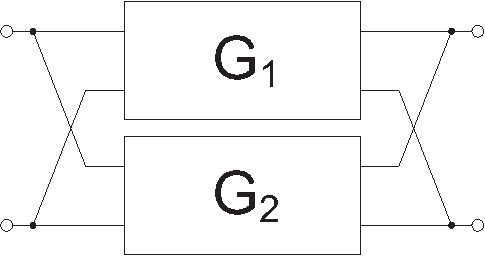
\includegraphics[width=0.2\textwidth]{img/Zweitor_Parallel} & 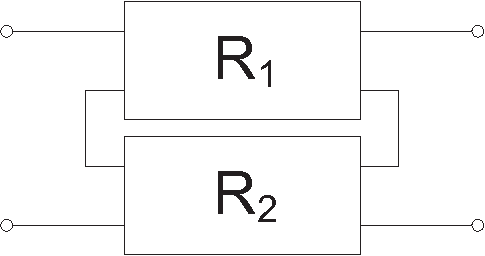
\includegraphics[width=0.2\textwidth]{img/Zweitor_Seriell} \\
	$\textbf{G}_{ges}=\textbf{G}_1+\textbf{G}_2$ & $\textbf{R}_{ges}=\textbf{R}_1+\textbf{R}_2$
\\&\\
	\textbf{Hybride Verschaltung} & \textbf{Inverse hybride Verschaltung}\\
	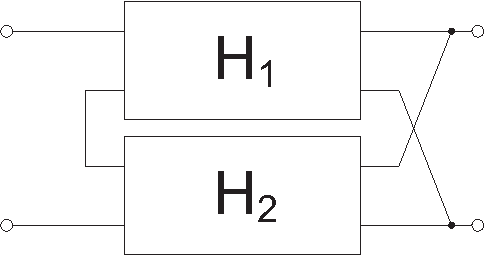
\includegraphics[width=0.2\textwidth]{img/Zweitor_Hybrid} & 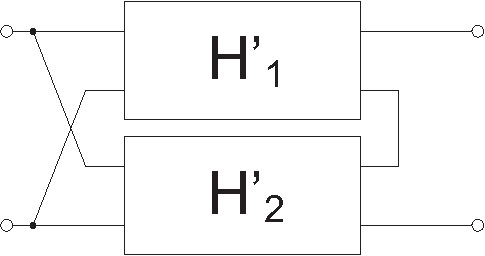
\includegraphics[width=0.2\textwidth]{img/Zweitor_inversHybrid} \\
	$\textbf{H}_{ges}=\textbf{H}_1+\textbf{H}_2$ & $\textbf{H'}_{ges}=\textbf{H'}_1+\textbf{H'}_2$
\\&\\
	\textbf{Kettenschaltung} & \textbf{Inverse Kettenschaltung}\\
	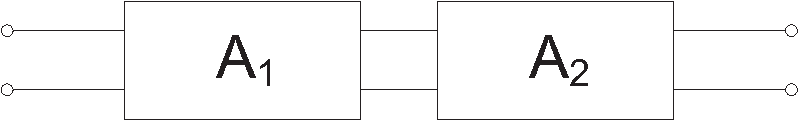
\includegraphics[width=0.21\textwidth, keepaspectratio]{img/Zweitor_Kette} &
	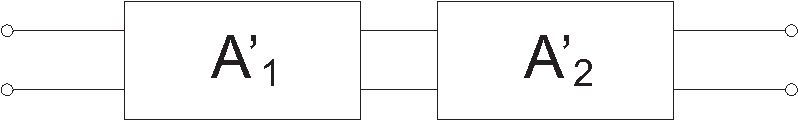
\includegraphics[width=0.21\textwidth]{img/Zweitor_inversKette}\\
	$\textbf{A}_{ges}=\textbf{A}_1\cdot \textbf{A}_2$ &
	$\textbf{A'}_{ges}=\textbf{A'}_2\cdot \textbf{A'}_1$
\end{tabular}

\subsection*{Umrechnung der Zweitor-Matrizen}
\subsubsection*{Implizit $\rightarrow$ explizit}
\begin{minipage}[b]{0.23\textwidth}
$\begin{bmatrix}\textbf{M} & \textbf{N}\end{bmatrix}\cdot \left.\begin{matrix}\underline{u}\\\underline{i}\end{matrix}\right]=\underline{0}\;\;\;\;\;|M^{-1}\cdot$\\\\
$\underline{u}+\textbf{M}^{-1}\textbf{N}\cdot \underline{i}=\underline{0}$\\\\
$\underline{u}=\underbrace{-\textbf{M}^{-1}\textbf{N}}_{\textbf{R}}\cdot \underline{i}$\\\\
\end{minipage}
\hfill
\begin{minipage}[b]{0.23\textwidth}
$\begin{bmatrix}\textbf{M} & \textbf{N}\end{bmatrix}\cdot \left.\begin{matrix}\underline{u}\\\underline{i}\end{matrix}\right]=\underline{0}\;\;\;\;\;|N^{-1}\cdot$\\\\
$\textbf{N}^{-1}\textbf{M}\cdot\underline{u}+ \underline{i}=\underline{0}$\\\\
$\underline{i}=\underbrace{-\textbf{N}^{-1}\textbf{M}}_{\textbf{G}}\cdot \underline{u}$\\\\
\end{minipage}

\subsubsection*{Explizit $\rightarrow$ implizit}
\begin{minipage}[b]{0.23\textwidth}
$\underline{u}=\textbf{R}\cdot \underline{i}$\\\\
$\underbrace{\textbf{1}}_{\textbf{M}}\cdot \underline{u}\underbrace{-\textbf{R}}_{\textbf{N}}\cdot \underline{i}=\underline{0}$
\end{minipage}
\hfill
\begin{minipage}[b]{0.23\textwidth}
$\underline{i}=\textbf{G}\cdot \underline{u}$\\\\
$\underbrace{-\textbf{G}}_{\textbf{M}}\cdot \underline{u}+\underbrace{\textbf{1}}_{\textbf{N}}\cdot \underline{i}=\underline{0}$
\end{minipage}

\subsubsection*{Parametrisiert $\rightarrow$ explizit}
$\left.\begin{matrix}\underline{u}\\\underline{i}\end{matrix}\right]=\begin{bmatrix}\textbf{U} \\ \textbf{I}\end{bmatrix}\cdot \underline{c}\;\;\;\;\;\Rightarrow\;\;\;\;\; \begin{matrix}\underline{u}\\\underline{i}\end{matrix}=\begin{matrix}\textbf{U}\\ \textbf{I}\end{matrix} \begin{matrix}\cdot\underline{c}\\ \cdot\underline{c}\end{matrix}$\\\\
\begin{minipage}[b]{0.23\textwidth}
$\underline{i}=\textbf{I}\cdot \underline{c}\;\;\;\;\;|\textbf{I}^{-1}\cdot$\\\\
$\Rightarrow \textbf{I}^{-1}\cdot \underline{i}=\underline{c}$\\\\
$\Rightarrow \underline{u}=\underbrace{\textbf{U}\cdot \textbf{I}^{-1}}_{R}\cdot \underline{i}$
\end{minipage}
\hfill
\begin{minipage}[b]{0.23\textwidth}
$\underline{u}=\textbf{U}\cdot \underline{c}\;\;\;\;\;|\textbf{U}^{-1}\cdot$\\\\
$\Rightarrow \textbf{U}^{-1}\cdot \underline{u}=\underline{c}$\\\\
$\Rightarrow \underline{i}=\underbrace{\textbf{I}\cdot \textbf{U}^{-1}}_{G}\cdot \underline{u}$
\end{minipage}

\subsubsection*{Explizit $\rightarrow$ parametrisiert}
\begin{minipage}[b]{0.23\textwidth}
$\underline{u}=\textbf{R}\cdot \underline{i}$\\\\
$\textbf{U}=\textbf{R};\;\;\;\;\;\;\textbf{I}=\textbf{1}$
\end{minipage}
\hfill
\begin{minipage}[b]{0.23\textwidth}
$\underline{i}=\textbf{G}\cdot \underline{u}$\\\\
$\textbf{U}=\textbf{1};\;\;\;\;\;\;\textbf{I}=\textbf{G}$
\end{minipage}

\subsubsection*{Implizit $\rightarrow$ parametrisiert}
$\textbf{U}=-\textbf{M}^{-1}\textbf{N};\;\;\; \textbf{I}=\textbf{1}\;\;\;$ oder $\;\;\;\textbf{U}=\textbf{1};\;\;\; \textbf{I}=-\textbf{N}^{-1}\textbf{M}$

\subsubsection*{Parametrisiert $\rightarrow$ implizit}
$\textbf{M}=-\textbf{I}\cdot\textbf{U}^{-1};\;\;\; \textbf{N}=\textbf{1}\;\;\;$ oder $\;\;\;\textbf{M}=\textbf{1};\;\;\; \textbf{N}=-\textbf{U}\cdot\textbf{I}^{-1}$

\subsubsection*{Explizit $\rightarrow$ explizit}
\begin{minipage}[b]{0.23\textwidth}
$\underline{i}=\textbf{G}\cdot \underline{u}+\underline{I}_0\;\;\;|\textbf{R}\cdot$\\\\
$\textbf{R}\cdot \underline{i}=\underbrace{\textbf{R}\cdot\textbf{G}}_{\textbf{1}}\cdot \underline{u}+\textbf{R}\cdot\underline{I}_0$\\\\
$\underline{u}=\textbf{R}\cdot\underline{i}-\textbf{R}\cdot\underline{I}_0$
\end{minipage}
\hfill
\begin{minipage}[b]{0.23\textwidth}
$\underline{u}=\textbf{R}\cdot \underline{i}+\underline{U}_0\;\;\;|\textbf{G}\cdot$\\\\
$\textbf{G}\cdot \underline{u}=\underbrace{\textbf{G}\cdot\textbf{R}}_{\textbf{1}}\cdot \underline{i}+\textbf{G}\cdot\underline{U}_0$\\\\
$\underline{i}=\textbf{G}\cdot\underline{u}-\textbf{G}\cdot\underline{U}_0$
\end{minipage}\\\\

{\small\begin{tabular}{@{}|@{}c@{}|@{}c@{}|@{}c@{}|@{}c@{}|}
\hline & \textbf{R} & \textbf{G} & \textbf{H}\\
\hline \textbf{R} & $\begin{bmatrix}r_{11} & r_{12}\\ r_{21} & r_{22}\end{bmatrix}$ & $\frac{1}{det(\textbf{G})}\begin{bmatrix}g_{22} & -g_{12}\\ -g_{21} & g_{11}\end{bmatrix}$ & $\frac{1}{h_{22}}\begin{bmatrix}det(\textbf{H}) & h_{12}\\ -h_{21} & 1\end{bmatrix}$\\
\hline \textbf{G} & $\frac{1}{det(\textbf{R})}\begin{bmatrix}r_{22} & -r_{12}\\ -r_{21} & r_{11}\end{bmatrix}$ & $\begin{bmatrix}g_{11} & g_{12}\\ g_{21} & g_{22}\end{bmatrix}$ & $\frac{1}{h_{11}}\begin{bmatrix}1 & -h_{12}\\ h_{21} & det(\textbf{H})\end{bmatrix}$\\
\hline \textbf{H} & $\frac{1}{r_{22}}\begin{bmatrix}det(\textbf{R}) & r_{12}\\ -r_{21} & 1\end{bmatrix}$ & $\frac{1}{g_{11}}\begin{bmatrix}1 & -g_{12}\\ g_{21} & det(\textbf{G})\end{bmatrix}$ & $\begin{bmatrix}h_{11} & h_{12}\\ h_{21} & h_{22}\end{bmatrix}$\\
\hline \textbf{H'} & $\frac{1}{r_{11}}\begin{bmatrix}1 & -r_{12}\\ r_{21} & det(\textbf{R})\end{bmatrix}$ & $\frac{1}{g_{22}}\begin{bmatrix}det(\textbf{G}) & g_{12}\\ -g_{21} & 1\end{bmatrix}$ & $\frac{1}{det(\textbf{H})}\begin{bmatrix}h_{22} & -h_{12}\\ -h_{21} & h_{11}\end{bmatrix}$\\
\hline \textbf{A} & $\frac{1}{r_{21}}\begin{bmatrix}r_{11} & det(\textbf{R})\\ 1 & r_{22}\end{bmatrix}$ & $\frac{1}{g_{21}}\begin{bmatrix}-g_{22} & -1\\ -det(\textbf{G}) & -g_{11}\end{bmatrix}$ & $\frac{1}{h_{21}}\begin{bmatrix}-det(\textbf{H}) & -h_{11}\\ -h_{22} & -1\end{bmatrix}$\\
\hline \textbf{A'} & $\frac{1}{r_{12}}\begin{bmatrix}r_{22} & det(\textbf{R})\\ 1 & r_{11}\end{bmatrix}$ & $\frac{1}{g_{12}}\begin{bmatrix}-g_{11} & -1\\ -det(\textbf{G}) & -g_{22}\end{bmatrix}$ & $\frac{1}{h_{12}}\begin{bmatrix}1 & h_{11}\\ h_{22} & det(\textbf{H})\end{bmatrix}$\\
\hline 
\end{tabular}}\\\\\\
{\small\begin{tabular}{@{}|@{}c@{}|@{}c@{}|@{}c@{}|@{}c@{}|}
\hline & \textbf{H'} & \textbf{A} & \textbf{A'}\\
\hline \textbf{R} & $\frac{1}{h'_{11}}\begin{bmatrix}1 & -h'_{12}\\ h'_{21} & det(\textbf{H}')\end{bmatrix}$ & $\frac{1}{a_{21}}\begin{bmatrix}a_{11} & det(\textbf{A})\\ 1 & a_{22}\end{bmatrix}$ & $\frac{1}{a'_{21}}\begin{bmatrix}a'_{22} & 1\\ det(\textbf{A'}) & a'_{11}\end{bmatrix}$\\
\hline \textbf{G} & $\frac{1}{h'_{22}}\begin{bmatrix}det(\textbf{H}') & h'_{12}\\ -h'_{21} & 1\end{bmatrix}$ & $\frac{1}{a_{12}}\begin{bmatrix}a_{22} & -det(\textbf{A})\\ -1 & a_{11}\end{bmatrix}$ & $\frac{1}{a'_{12}}\begin{bmatrix}a'_{11} & -1\\ -det(\textbf{A}') & a'_{22}\end{bmatrix}$\\
\hline \textbf{H} & $\frac{1}{det(\textbf{H}')}\begin{bmatrix}h'_{22} & -h'_{12}\\ -h'_{21} & h'_{11}\end{bmatrix}$ & $\frac{1}{a_{22}}\begin{bmatrix}a_{12} & det(\textbf{A})\\ -1 & a_{21}\end{bmatrix}$ & $\frac{1}{a'_{11}}\begin{bmatrix}a'_{12} & 1\\ -det(\textbf{A}') & a'_{21}\end{bmatrix}$\\
\hline \textbf{H'} & $\begin{bmatrix}h'_{11} & h'_{12}\\ h'_{21} & h'_{22}\end{bmatrix}$ & $\frac{1}{a_{11}}\begin{bmatrix}a_{21} & -det(\textbf{A})\\ 1 & a_{12}\end{bmatrix}$ & $\frac{1}{a'_{22}}\begin{bmatrix}a'_{21} & -1\\ det(\textbf{A}') & a'_{12}\end{bmatrix}$\\
\hline \textbf{A} & $\frac{1}{h'_{21}}\begin{bmatrix}1 & h'_{22}\\ h'_{11} & det(\textbf{H}')\end{bmatrix}$ & $\begin{bmatrix}a_{11} & a_{12}\\ a_{21} & a_{22}\end{bmatrix}$ & $\frac{1}{det(\textbf{A}')}\begin{bmatrix}a'_{22} & a'_{12}\\ a'_{21} & a'_{11}\end{bmatrix}$\\
\hline \textbf{A'} & $\frac{1}{h'_{12}}\begin{bmatrix}-det(\textbf{H}') & -h'_{22}\\ -h'_{11} & -1\end{bmatrix}$ & $\frac{1}{det(\textbf{A})}\begin{bmatrix}a_{22} & a_{12}\\ a_{21} & a_{11}\end{bmatrix}$ & $\begin{bmatrix}a'_{11} & a'_{12}\\ a'_{21} & a'_{22}\end{bmatrix}$\\
\hline 
\end{tabular}}

\subsection*{Spezielle Zweitore}
\subsubsection*{VCCS Spannungsgesteuerte Stromquelle}
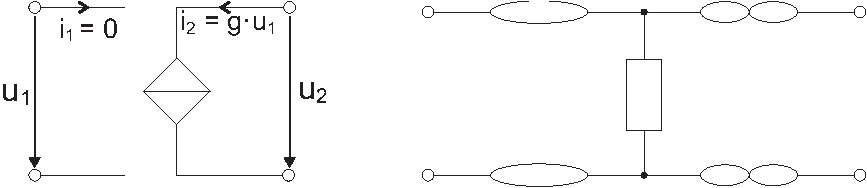
\includegraphics[width=0.45\textwidth]{img/OP_USI}\\\\
\begin{tabular}{ll}
$\textbf{A}=\begin{bmatrix}0 & -\frac{1}{g}\\ 0 & 0\end{bmatrix}\;\;\textbf{G}=\begin{bmatrix}0 & 0\\ g & 0\end{bmatrix}\;\;\textbf{M}=\begin{bmatrix}0 & 0\\ -g & 0\end{bmatrix}\;\;\textbf{N}=\begin{bmatrix}1 & 0\\ 0 & 1\end{bmatrix}$
\end{tabular}

\subsubsection*{CCCS Stromggesteuerte Stromquelle}
\begin{minipage}[b]{0.23\textwidth}
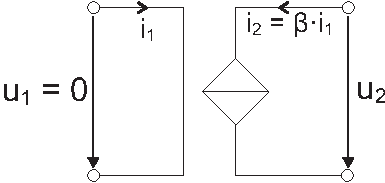
\includegraphics[width=0.95\textwidth]{img/OP_ISI}
\end{minipage}
\hfill
\begin{minipage}[b]{0.23\textwidth}
\begin{tabular}{ll}
$\textbf{A}=\begin{bmatrix}0 & 0\\ 0 & -\frac{1}{\beta}\end{bmatrix}\;\;\textbf{H}=\begin{bmatrix}0 & 0\\ \beta & 0\end{bmatrix}$
\end{tabular}\\\\
\end{minipage}

\subsubsection*{VCVS Spannungsgesteurte Spannungsquelle}
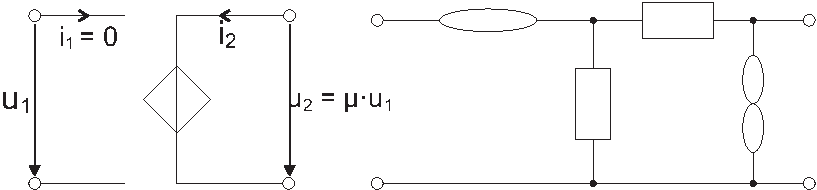
\includegraphics[width=0.45\textwidth]{img/OP_USU}\\\\
\begin{tabular}{ll}
$\textbf{A}=\begin{bmatrix}\frac{1}{\mu} & 0\\ 0 & 0\end{bmatrix}\;\;\textbf{H'}=\begin{bmatrix}0 & 0\\ \mu & 0\end{bmatrix}$
\end{tabular}

\subsubsection*{CCVS Stromgesteuerte Spannungsquelle}
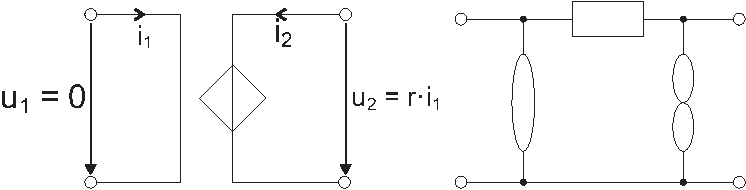
\includegraphics[width=0.45\textwidth]{img/OP_ISU}\\\\
\begin{tabular}{ll}
$\textbf{A}=\begin{bmatrix}0 & 0\\ \frac{1}{r} & 0\end{bmatrix}\;\;\textbf{R}=\begin{bmatrix}0 & 0\\ r & 0\end{bmatrix}\;\;\textbf{M}=\begin{bmatrix}1 & 0\\ 0 & 1\end{bmatrix}\;\;\textbf{N}=\begin{bmatrix}0 & 0\\ -r & 0\end{bmatrix}$
\end{tabular}

\subsubsection*{Nullor}
Quellenfrei, streng linear, nicht verlustlos\\\\
\begin{minipage}[b]{0.13\textwidth}
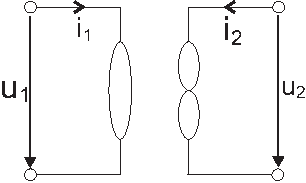
\includegraphics[width=0.95\textwidth]{img/OP_Nullor}
\end{minipage}
\hfill
\begin{minipage}[b]{0.33\textwidth}
\begin{tabular}{ll}
$\textbf{A}=\begin{bmatrix}0 & 0\\ 0 & 0\end{bmatrix}\;\;\textbf{M}=\begin{bmatrix}1 & 0\\ 0 & 0\end{bmatrix}\;\;\textbf{N}=\begin{bmatrix}0 & 0\\ 1 & 0\end{bmatrix}$
\end{tabular}\\
\end{minipage}

\subsubsection*{Gyrator}
Dualwandler, Positiv-Immittanz-Inverter (PII)\\\\
\begin{minipage}[b]{0.2\textwidth}
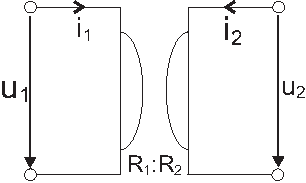
\includegraphics[width=0.9\textwidth]{img/OP_Gyrator}
\end{minipage}
\hfill
\begin{minipage}[b]{0.26\textwidth}
Verlustlos ($R_1=R_2=R_d$)\\
Pfeilrichtung $\rightarrow$ für $R_d$\\
$\textbf{G}=-\textbf{G}^T$\\
$\textbf{R}=-\textbf{R}^T$\\
$det(\textbf{A})=det(\textbf{A}')=-1$\\
$F_{Gyr}=F^d$
\end{minipage}\\

\begin{tabular}{lll}
$\textbf{G}=\begin{bmatrix}0 & \frac{1}{R_2}\\ -\frac{1}{R_1} & 0\end{bmatrix}$ & $\textbf{R}=\begin{bmatrix}0 & -R_1\\ R_2 & 0\end{bmatrix}$ & $\textbf{A}=\begin{bmatrix}0 & R_1\\ \frac{1}{R_2} & 0\end{bmatrix}$\\\\
$\textbf{A'}=\begin{bmatrix}0 & -R_2\\ -\frac{1}{R_1} & 0\end{bmatrix}$ & $\textbf{N}=\begin{bmatrix}0 & R_1\\ -R_2 & 0\end{bmatrix}$ & $\textbf{M}=\begin{bmatrix}1 & 0\\ 0 & 1\end{bmatrix}$
\end{tabular}

\subsubsection*{Idealer Übertrager}
Positiv-Immittanz-Konverter (PIK)\\\\
\begin{minipage}[b]{0.2\textwidth}
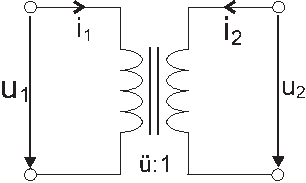
\includegraphics[width=0.9\textwidth]{img/OP_Uebertrager}
\end{minipage}
\hfill
\begin{minipage}[b]{0.26\textwidth}
Verlustlos\\
Reziprok\\
Umkehrbar für ü $=\pm 1$\\
$det(\textbf{A})=det(\textbf{A}')=1$\\
\end{minipage}\\

\begin{tabular}{lll}
$\textbf{A}=\begin{bmatrix}\ddot{u} & 0\\ 0 & \frac{1}{\ddot{u}}\end{bmatrix}$ & $\textbf{A'}=\begin{bmatrix}\frac{1}{\ddot{u}} & 0\\ 0 & \ddot{u}\end{bmatrix}$ & $\textbf{H}=\begin{bmatrix}0 & \ddot{u}\\ -\ddot{u} & 0\end{bmatrix}$\\\\
$\textbf{H'}=\begin{bmatrix}0 & -\frac{1}{\ddot{u}}\\ \frac{1}{\ddot{u}} & 0\end{bmatrix}$ & $\textbf{M}=\begin{bmatrix}1 & -\ddot{u}\\ 0 & 0\end{bmatrix}$ & $\textbf{N}=\begin{bmatrix}0 & 0\\ \ddot{u} & 1\end{bmatrix}$
\end{tabular}

\subsubsection*{NIK}
Negativ-Immittanz-Konverter (NIK)\\\\
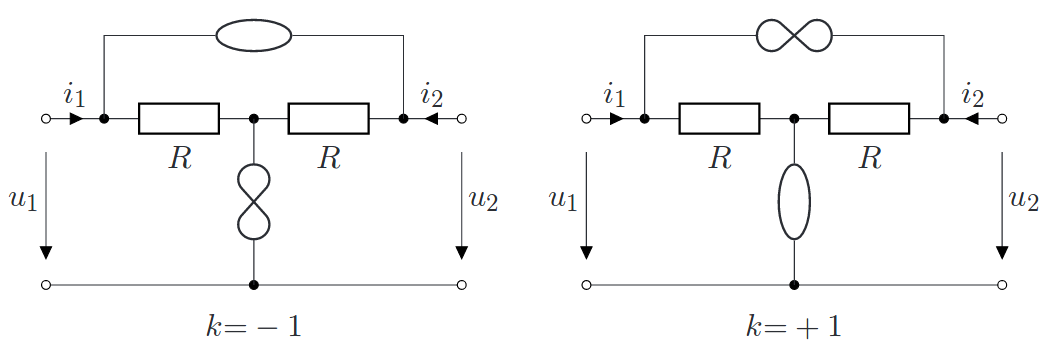
\includegraphics[width=1\linewidth, keepaspectratio]{img/NIK.png}
Aktiv, antireziprok, für $|k|=1$ symmetrisch\\\\
\begin{tabular}{ll}
$k=1$ & $F$ ist an der $i_1$-Achse gespiegelter Zweipol\\
$k=-1$ & $F$ ist an der $u_1$-Achse gespiegelter Zweipol\\\\
\end{tabular}
\begin{tabular}{lll}
$\textbf{A}=\begin{bmatrix}-k & 0\\ 0 & \frac{1}{k}\end{bmatrix}$ & $\textbf{A'}=\begin{bmatrix}-\frac{1}{k} & 0\\ 0 & k\end{bmatrix}$ & $\textbf{H}=\begin{bmatrix}0 & -k\\ -k & 0\end{bmatrix}$\\\\
$\textbf{H'}=\begin{bmatrix}0 & -\frac{1}{k}\\ -\frac{1}{k} & 0\end{bmatrix}$ & $\textbf{M}=\begin{bmatrix}1 & k\\ 0 & 0\end{bmatrix}$ & $\textbf{N}=\begin{bmatrix}0 & 0\\ 1 & \frac{1}{k}\end{bmatrix}$
\end{tabular}

\section*{Bipolar-Transistoren}
\subsection*{Kennlinien eines npn-Transistors}
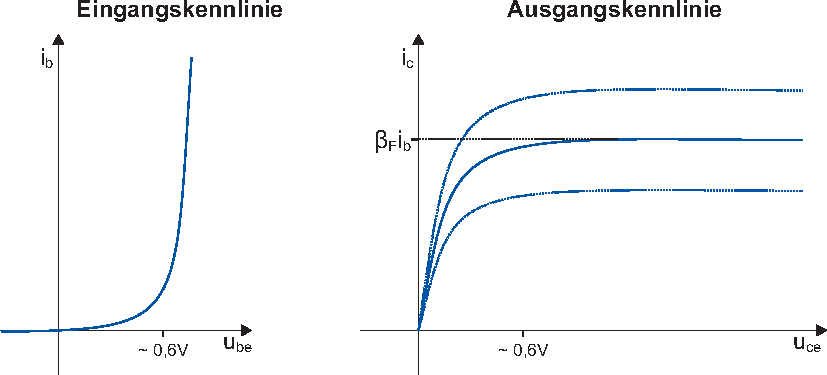
\includegraphics[width=0.4\textwidth]{img/Kennlinie_Transistor}
\subsection*{Basisschaltung}
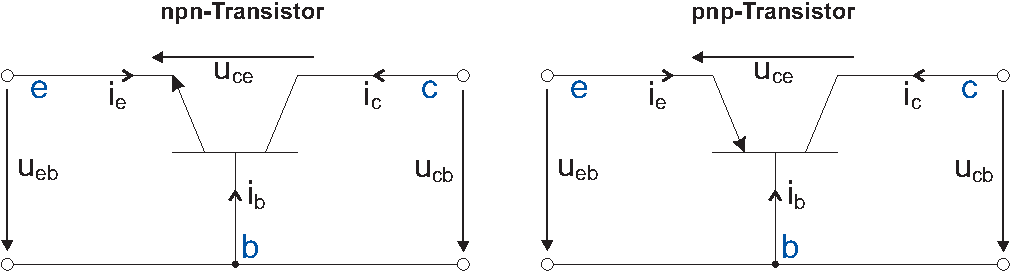
\includegraphics[width=0.4\textwidth]{img/Transistor_Basisschaltung}
\subsection*{Emitterschaltung}
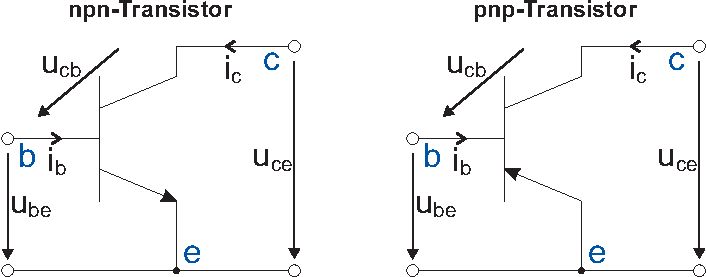
\includegraphics[width=0.4\textwidth]{img/Transistor_Emitterschaltung}

\subsection*{Ebers-Moll-Modell (Basisschaltung, npn)}
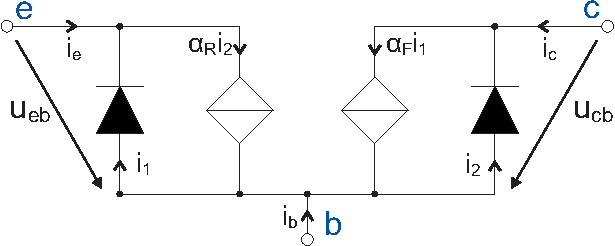
\includegraphics[width=0.4\textwidth]{img/Ebers-Moll}\\\\
$i_e=-I_{es}\cdot (e^{-\frac{u_{eb}}{U_T}}-1)+\alpha_RI_{cs}\cdot (e^{-\frac{u_{cb}}{U_T}}-1)$\\\\
$i_c=\alpha_FI_{es}\cdot (e^{-\frac{u_{eb}}{U_T}}-1)-I_{cs}\cdot (e^{-\frac{u_{cb}}{U_T}}-1)$

\subsection*{Vereinfachung für Vorwärtsbetrieb (npn)}
\textbf{Bedingung} für den Vorwärtsbetrieb: $u_{be}>0 \wedge u_{cb}\geq 0$
\subsubsection*{Basisschaltung}
\begin{minipage}[b]{0.23\textwidth}
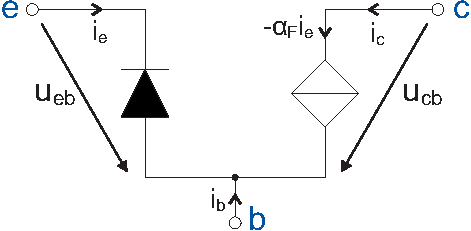
\includegraphics[width=\textwidth]{img/Basisschaltung_Vereinfachung}\\
\end{minipage}
\hfill
\begin{minipage}[b]{0.23\textwidth}
$i_e=-I_{es}\cdot (e^{-\frac{u_{eb}}{U_T}}-1)$\\\\
$i_c=-\alpha_Fi_e$\\\\
\end{minipage}

\subsubsection*{Emitterschaltung}
\begin{minipage}[b]{0.23\textwidth}
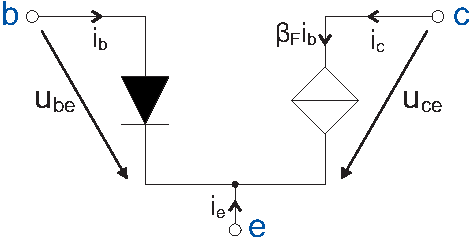
\includegraphics[width=\textwidth]{img/Emitterschaltung_Vereinfachung}\\
\end{minipage}
\hfill
\begin{minipage}[b]{0.23\textwidth}
$i_b=\overbrace{\underbrace{(1-\alpha_F)}_{\approx \frac{1}{\beta_F}}\cdot I_{es}}^{\approx I_S}\cdot (e^{\frac{u_{be}}{U_T}}-1)$\\\\
$i_c=\beta_Fi_b$\\\\
$i_c=\overbrace{\underbrace{\alpha_F}_{\approx 1}\cdot I_{es}}^{\approx \beta_F\cdot I_S}\cdot (e^{\frac{u_{be}}{U_T}}-1)$\\
\end{minipage}


\subsection*{Linearisierung}
(Emitterschaltung, Vorwärtsbetrieb, npn)\\\\
\begin{minipage}[t]{0.23\textwidth}
Großsignal-ESB:\\\\
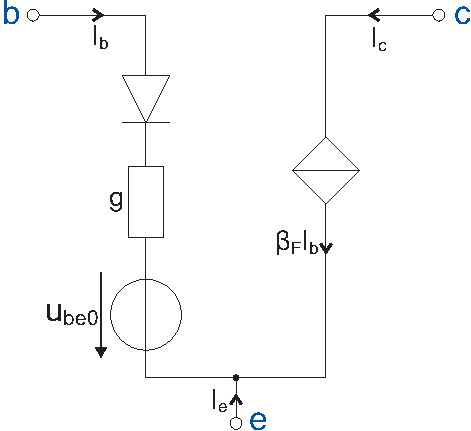
\includegraphics[width=\textwidth]{img/Transistor_GSE}\\\\
\end{minipage}
\hfill
\begin{minipage}[t]{0.23\textwidth}
Kleinsignal-ESB:\\\\
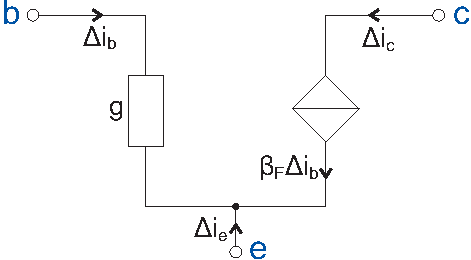
\includegraphics[width=\textwidth]{img/Transistor_KSE}\\\\
\end{minipage}\\

\begin{minipage}[t]{0.23\textwidth}
$\beta_F=\frac{i_c}{i_b}=\frac{\alpha_F}{1-\alpha_F}$\\\\
$\alpha_F=\frac{\beta_F}{1+\beta_F}$\\\\
$g=\left.\frac{\partial i_b}{\partial u_{be}}\right|_{AP}\approx -\frac{I_e}{\beta_F\cdot U_T}$\\\\
$g\approx \frac{I_b}{U_T}=\frac{I_c}{\beta_F\cdot U_T}$\\\\
\end{minipage}
\hfill
\begin{minipage}[t]{0.23\textwidth}
Wenn $\beta_F \rightarrow \infty$:\\\\
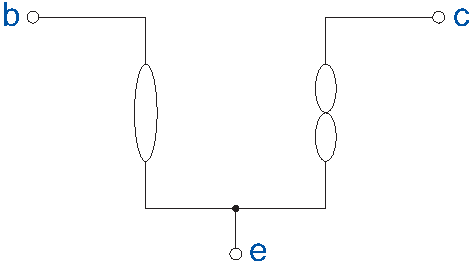
\includegraphics[width=\textwidth]{img/Nullormodell}
Dreipol Nullor $\textbf{A}=\begin{bmatrix}0 & 0\\ 0 & 0\end{bmatrix}$. Wie normaler Nullor.
\end{minipage}

\section*{Feldeffekt-Transistoren (FET)}
\subsection*{nMOS}

\begin{minipage}[b]{0.35\textwidth}
Guter Pull-Down\\
Source am niedrigeren Potential ($u_{DS} > 0$)
\end{minipage}
\hfill
\begin{minipage}[b]{0.1\textwidth}
\centering
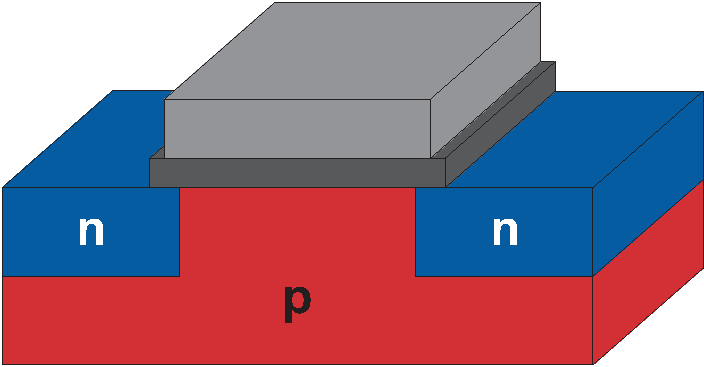
\includegraphics[width=\textwidth]{img/nMOS}
\end{minipage}

\begin{itemize}[label=,leftmargin=0mm]
	\item $i_G=0A$
	\item $i_D=\begin{cases}
				0 & u_{GS} < U_t (aus) \\
				& \wedge \; u_{DS} \geq 0 \\
				\beta\left(u_{GS}-U_t-\frac{u_{DS}}{2}\right)u_{DS} & u_{GS} > U_t $ (linear)$ \\
				& \wedge \;0 < u_{DS} < u_{GS}-U_t \\
				\frac{\beta}{2}\left(u_{GS}-U_t\right)^2 & u_{GS} > U_t $ (Sättigung)$\\
				& \wedge \;0 < u_{GS}-U_t < u_{DS} \\
			\end{cases}$
\end{itemize}
Enhancement-Typ (selbssperrend): $U_t \approx 1V$\\
Depletion-Typ (selbstleitend): $U_t \approx -1V$\\\\
\textbf{Kanallängenmodulation:} $i_D'=i_D\cdot (1+\lambda \cdot u_{DS})$

\subsection*{pMOS}

\begin{minipage}[b]{0.35\textwidth}
Guter Pull-Up\\
Source am höheren Potential ($u_{DS} < 0$)
\end{minipage}
\hfill
\begin{minipage}[b]{0.1\textwidth}
\centering
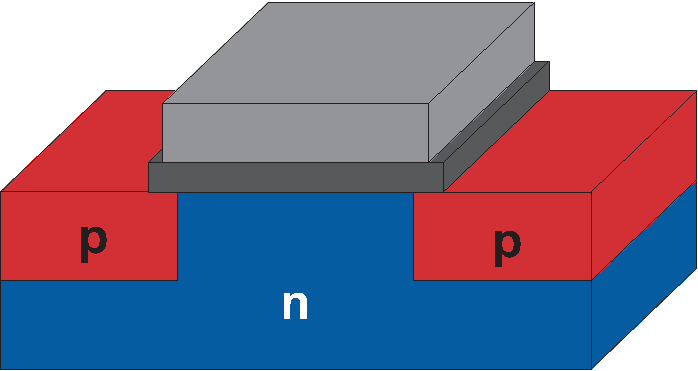
\includegraphics[width=\textwidth]{img/pMOS}
\end{minipage}

\begin{itemize}[label=,leftmargin=0mm]
	\item $i_G=0A$
	\item $i_D=\begin{cases}
				0 & u_{GS} > U_t (aus) \\
				& \wedge \; u_{DS} \leq 0 \\
				-\beta\left(u_{GS}-U_t-\frac{u_{DS}}{2}\right)u_{DS} & u_{GS} < U_t $ (linear)$ \\
				& \wedge \;0 > u_{DS} > u_{GS}-U_t \\
				\frac{-\beta}{2}\left(u_{GS}-U_t\right)^2 & u_{GS} < U_t $ (Sättigung)$\\
				& \wedge \;0 > u_{GS}-U_t > u_{DS} \\
			\end{cases}$
\end{itemize}
Enhancement-Typ (selbstsperrend): $U_t \approx -1V$\\\\
\textbf{Kanallängenmodulation:} $i_D'=i_D\cdot (1-\lambda \cdot u_{DS})$

\subsection*{Kleinsignal-Ersatzschaltbilder (nMOS)}
\subsubsection*{Linearer Bereich}
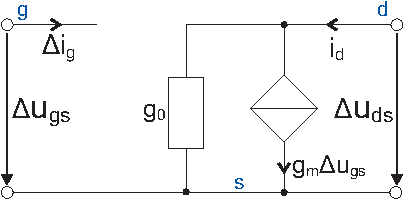
\includegraphics[width=0.30\textwidth]{img/FET_KSE_lin}\\\\
$g_m=\left.\frac{\partial i_d}{\partial u_{gs}}\right|_{AP}=\beta \cdot U_{ds}$\\\\
$g_0=\left.\frac{\partial i_d}{\partial u_{ds}}\right|_{AP}=\beta \cdot (U_{gs}-U_T-U_{ds})$

\subsubsection*{Sättigungsbereich}
\begin{minipage}[b]{0.25\textwidth}
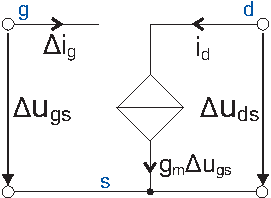
\includegraphics[width=0.9\textwidth]{img/FET_KSE_sat}
\end{minipage}
\hfill
\begin{minipage}[b]{0.2\textwidth}
$g_m=\left.\frac{\partial i_d}{\partial u_{gs}}\right|_{AP}$\\\\
$g_m=\beta \cdot (U_{gs}-U_T)$\\\\
\end{minipage}

\section*{Operationsverstärker}
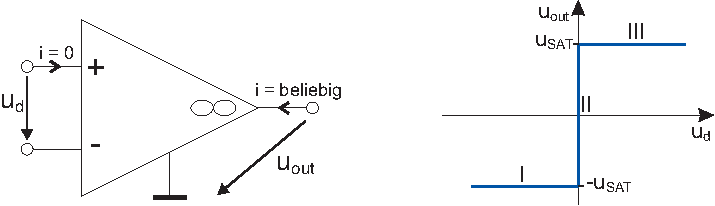
\includegraphics[width=0.45\textwidth]{img/OP}\\\\
Operationsverstärker müssen immer über ihren invertierenden Eingang rückgekoppelt werden, da sich sonst eine Z-Kennlinie ergibt und der Arbeitspunkt somit nicht mehr eindeutig ist.
\subsection*{Ersatzschaltbilder}
\textbf{$u_d$ mit einzeichnen.}
\subsubsection*{ESB I}
\begin{minipage}[b]{0.3\textwidth}
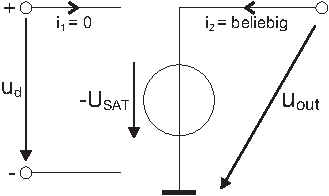
\includegraphics[width=0.9\textwidth]{img/OP_ESBI}
\end{minipage}
\hfill
\begin{minipage}[b]{0.16\textwidth}
$u_d<0$\\\\
$u_{out}=-U_{SAT}$
\end{minipage}

\subsubsection*{ESB II}
\begin{minipage}[b]{0.3\textwidth}
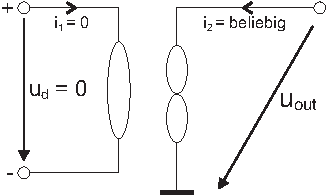
\includegraphics[width=0.9\textwidth]{img/OP_ESBII}
\end{minipage}
\hfill
\begin{minipage}[b]{0.16\textwidth}
$u_d=0$\\\\
$|u_{out}|\leq |U_{SAT}|$
\end{minipage}

\subsubsection*{ESB III}
\begin{minipage}[b]{0.3\textwidth}
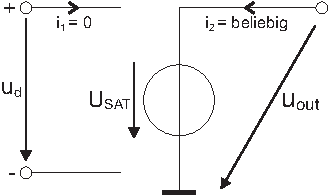
\includegraphics[width=0.9\textwidth]{img/OP_ESBIII}
\end{minipage}
\hfill
\begin{minipage}[b]{0.16\textwidth}
$u_d>0$\\\\
$u_{out}=U_{SAT}$
\end{minipage}

\subsection*{OP-Schaltungen}
\subsubsection*{Spannungsfolger (Impedanzwandler)}
\begin{minipage}[b]{0.3\textwidth}
\includegraphics[width=0.9\textwidth]{img/OP_SF}
\end{minipage}
\hfill
\begin{minipage}[b]{0.16\textwidth}
$u_{out}=u_{in}$\\\\
$v_u=1$
\end{minipage}

\begin{tabular}{c|c}
	Nichtinvertierender Verstärker & Invertierender Verstärker\\
	\includegraphics[width=0.2\textwidth]{img/OP_NiV} &
	\includegraphics[width=0.2\textwidth]{img/OP_IV}\\
	$u_{out}=(1+\frac{R_0}{R_1})\cdot u_{in}$ & $u_{out}=-\frac{R_0}{R_1}\cdot u_{in}$\\
	$v_u=1+\frac{R_0}{R_1}$ & $v_u=\frac{R_0}{R_1}$
\end{tabular}


\begin{tabular}{c|c}
	Differenzierer & Integrierer\\
	\includegraphics[width=0.2\textwidth]{img/OP_Diff} & \includegraphics[width=0.2\textwidth]{img/OP_Int}\\
	$u_{out}=-RC\cdot \dot{u}_{in}$ & 
	$u_{out}=-u_c(t_0)-\frac{1}{RC}\cdot \int\limits_{t_0}^{t_1}u_{in}dt$
\end{tabular}

\subsubsection*{Differenzverstärker/Subtrahierer}
\begin{minipage}[b]{0.25\textwidth}
\includegraphics[width=\textwidth]{img/OP_PDiffV}
\end{minipage}
\hfill
\begin{minipage}[b]{0.2\textwidth}
Bedingung:\\
$R_1=R_3;\;\;R_2=R_4$\\\\
$u_{out}=\frac{R_2}{R_1}\cdot (u_2-u_1)$\\\\
$u_{out}=\frac{R_4}{R_3}\cdot (u_2-u_1)$\\\\
\end{minipage}

\begin{tabular}{c|c}
	\emph{Logarithmierer} & \emph{Exponentierer}\\
	\includegraphics[width=0.2\textwidth]{img/OP_Log} & \includegraphics[width=0.2\textwidth]{img/OP_Exp}\\
	$u_{out}=-U_T\cdot ln(\frac{u_{in}}{R\cdot I_S})$ & 
	$u_{out}=-R\cdot I_S\cdot e^{\frac{u_{in}}{U_T}}$
\end{tabular}

\subsubsection*{Ideale Diode}
\begin{minipage}[b]{0.2\textwidth}
\includegraphics[width=\textwidth]{img/OP_IdealeDiode}
\end{minipage}

\begin{tabular}{c|c}
	\emph{Konkaver Widerstand} & \emph{Konvexer Widerstand}\\
\includegraphics[width=0.2\textwidth]{img/OP_Rkonkav} & \includegraphics[width=0.2\textwidth]{img/OP_Rkonvex}\\
$U_0<U_{SAT}$ & $I_0<G\cdot U_{SAT}$
\end{tabular}

\subsubsection*{VCVS Voltage Controlled Voltage Source}
\begin{tabular}{ll}
$\mu\geq 1$ & Nichtinvertierender Verstärker\\
$\mu<0$ & Spannungsfolger und invertierender Verstärker\\
& hintereinander\\
$0<\mu<1$ & Spannungsfolger und zwei invertierende\\
& Verstärker hintereinander
\end{tabular}

\subsubsection*{CCVS Current Controlled Voltage Source}
\begin{tabular}{ll}
$r<0$ & Invertierender Verstärker mit $R_1=0\Omega$\\
$r>0$ & Zusätzlich invertierenden Verstärker mit $v_u=-1$\\
& nachschalten
\end{tabular}

\subsubsection*{Gyrator}
\begin{itemize}[label=- ,leftmargin=5mm]
	\item Parallelschaltung zweier VCCS
	\item Serienschaltung zweier CCVS
	\item Kettenschaltung eines NIK ($k=-1$) mit einem NII
\end{itemize}

\section*{Knotenspannungsanalyse (KSA)}
$\textbf{Y}_k\cdot \underline{u}_k=\underline{i}_q$

\subsection*{1. Nichtspannungsgesteuerte Elemente ersetzen}
\subsubsection*{Ideale Spannungsquelle}
\begin{minipage}[b]{0.35\textwidth}
\includegraphics[width=\textwidth]{img/KSA_Quellwandlung}
\end{minipage}
\hfill
\begin{minipage}[b]{0.1\textwidth}
$I_0=\frac{U_0}{R}$\\\\
\end{minipage}\\\\
\includegraphics[width=0.48\textwidth]{img/KSA_Quellwandlung2}\\\\
$I_0=G\cdot U_0$
\subsubsection*{Idealer Übertrager}
\includegraphics[width=0.48\textwidth]{img/KSA_Uebertrager}
\subsubsection*{VCVS Voltage Controlled Voltage Source}
\includegraphics[width=0.48\textwidth]{img/KSA_USU}\\\\
$u_2=\mu \cdot u_1\;\;\;\;\;i_2=-\frac{\mu \cdot u_1}{R_D}$\\\\\\
\includegraphics[width=0.48\textwidth]{img/KSA_USU2}\\\\
$i_2=-G\cdot \mu\cdot u_1$
\subsubsection*{CCCS Current Controlled Current Source}
\includegraphics[width=0.48\textwidth]{img/KSA_ISI}\\\\
$i_2=\beta \cdot i_1\;\;\;\;\;u=R_d\cdot i_1\;\;\;\;\;i_2=\frac{\beta \cdot u}{R_d}$
\subsubsection*{CCVS Current Controlled Voltage Source}
\includegraphics[width=0.48\textwidth]{img/KSA_ISU}\\\\
$u_2=\beta \cdot i_1\;\;\;\;\;u=R_d\cdot i_1\;\;\;\;\;i_2=\frac{u}{R_d}\;\;\;\;\;u_2=-R_d\cdot i_1$

\subsection*{2. Knotenspannungsvektor $U_k$ aufstellen}
\subsection*{3. Knotenleitwertsmatrix $Y_k$ aufstellen}
\subsubsection*{Leitwert}
\begin{minipage}[b]{0.05\textwidth}
\includegraphics[width=\textwidth]{img/KSA_Widerstand}
\end{minipage}
\hfill
\begin{minipage}[b]{0.4\textwidth}
$\textbf{Y}_k=\;\;\begin{matrix}\begin{matrix} & & \;\;\;\kreis{$\alpha$} & \;\;\;\kreis{$\beta$} & \end{matrix}\\\begin{matrix} \; \\ \kreis{$\alpha$} \\ \kreis{$\beta$} \\ \; \end{matrix} \left[\begin{matrix} ... & ... & ... & ... \\ ... & G & -G & ... \\ ... & -G & G & ... \\ ...& ... & ... & ... \end{matrix}\right]\\ \; \end{matrix}$\\
\end{minipage}
\subsubsection*{Gyrator}
\begin{minipage}[b]{0.18\textwidth}
\includegraphics[width=\textwidth]{img/KSA_Gyrator}
\end{minipage}
\hfill
\begin{minipage}[b]{0.30\textwidth}
$\textbf{Y}_k=\;\;\begin{matrix}\begin{matrix} \;\;\; & \;\;\;\kreis{$\gamma$} & \;\;\kreis{$\delta$} & \;\kreis{$\alpha$} & \;\kreis{$\beta$} \end{matrix}\\\begin{matrix} \kreis{$\gamma$} \\ \kreis{$\delta$} \\ \kreis{$\alpha$} \\ \kreis{$\beta$} \end{matrix} \left[\begin{matrix}  &  & G & -G \\  &  & -G & G \\ -G & G & & \\ G & -G & & \end{matrix}\right]\\ \; \end{matrix}$\\
Wenn $\delta$ und $\beta$ auf GND sind:\\
$\textbf{Y}_k=\begin{matrix}\begin{matrix}\;\;\;\;\;\;\;\;\;\;\;\kreis{$\gamma$}&\;\;\;\kreis{$\alpha$} \end{matrix}\\\;\;\begin{matrix} \kreis{$\gamma$} \\ \kreis{$\alpha$} \end{matrix} \left[\begin{matrix} 0 & G \\-G & 0 \end{matrix}\right]
\end{matrix}$
\end{minipage}
\textbf{Pfeilrichtung wichtig.} 
$i_1=Gu_2$, $i_2=-Gu_1$
\subsubsection*{VCCS Voltage Controlled Current Source}
\begin{minipage}[b]{0.20\textwidth}
\includegraphics[width=\textwidth]{img/KSA_USI}
\end{minipage}
\hfill
\begin{minipage}[b]{0.28\textwidth}
$\textbf{Y}_k=\;\;\begin{matrix}\begin{matrix} & & \;\;\;\kreis{$\gamma$} & \;\;\;\kreis{$\delta$} & \end{matrix}\\\begin{matrix} \; \\ \kreis{$\alpha$} \\ \kreis{$\beta$} \\ \; \end{matrix} \left[\begin{matrix} ... & ... & ... & ... \\ ... & g_m & -g_m & ... \\ ... & -g_m & g_m & ... \\ ...& ... & ... & ... \end{matrix}\right]\\ \; \end{matrix}$\\
\end{minipage}

\subsection*{4. Quellvektor $I_q$ aufstellen}
\begin{minipage}[b]{0.10\textwidth}
\includegraphics[width=0.4\textwidth]{img/KSA_Stromquelle}
\end{minipage}
\hfill
\begin{minipage}[b]{0.30\textwidth}
$\textbf{I}_q=\;\;\begin{matrix} \; \\ \kreis{$\alpha$} \\ \kreis{$\beta$} \\ \; \end{matrix} \left[\begin{matrix} ... \\ I_0 \\ -I_0 \\ ... \end{matrix}\right]$\\
\end{minipage}

\subsection*{5. Reduzierte Knotenleitwertsmatrix $Y_k$}
\subsubsection*{Nullator}
In $\textbf{Y}_k$ die entsprechenden Spalten addieren und eine davon streichen \textbf{UND} entsprechenden Eintrag im $\underline{u}_k$-Vektor streichen.\\
Falls mit Masse verbunden: Spalte und $\underline{u}_k$-Eintrag streichen.
\subsubsection*{Norator}
In $\textbf{Y}_k$ die entsprechenden Zeilen addieren und eine davon streichen \textbf{UND} entsprechenden Eintrag im $\underline{i}_q$-Vektor streichen.\\
Falls mit Masse verbunden: Zeile und $\underline{i}_q$-Eintrag streichen.

\section*{Sonstiges}
\subsection*{Tellegenscher Satz}
Der Spannungsvektor steht immer senkrecht zum Stromvektor ($\textbf{A}\textbf{B}^T=\textbf{0}$ bzw. $\textbf{B}\textbf{A}^T=\textbf{0}$).

\subsection*{Tableau-Gleichungssystem}
$\begin{bmatrix}\textbf{B} & \textbf{0} \\ \textbf{0} & \textbf{A} \\ \textbf{M} & \textbf{N}\end{bmatrix}\cdot \left.\begin{matrix}\underline{u}\\\underline{i}\end{matrix}\right]=\left.\begin{matrix}\underline{0}\\ \underline{0} \\ \underline{e}\end{matrix}\right]$
Dimension $2b\times 2b$

\subsection*{Superpositionsprinzip}
Gilt für unabhängige Quellen in linearem Netzwerk für $u,i$.
\begin{enumerate}
	\item Jeweils alle Quellen bis auf eine auf Null setzen.
	\item Gesuchte Größe $u_{ai}$ berechnen.
	\item Resultierende Größe ist $u_a=u_{a1}+...+u_{an}$
	
\end{enumerate}
\subsection*{Substitutionsprinzip}
\begin{circuitikz}
	\draw(0,0)
	to[twoport, t=$\mathcal{N}_1$, v=$u$, i<=$i$] (0,2)
	to[short] (2,2)
	to[twoport, t=$\mathcal{N}_2$] (2,0)
	to[short] (0,0);
\end{circuitikz}
\\
\begin{tabular}{c|c}
	$\mathcal{N}_1$ Spannungsgesteuert & $\mathcal{N}_1$ Stromgesteuert\\
	\begin{circuitikz}
		\draw(0,0)
		to[twoport, t=$\mathcal{N}_1$, v=$u$, i<=$i$] (0,2)
		to[short] (2,2)
		to[V, v=$u$] (2,0)
		to[short] (0,0);
	\end{circuitikz} &
	\begin{circuitikz}
		\draw(0,0)
		to[twoport, t=$\mathcal{N}_1$, v=$u$, i<=$i$] (0,2)
		to[short] (2,2)
		to[I, i<^=$i$] (2,0)
		to[short] (0,0);
	\end{circuitikz}
\end{tabular}


\subsection*{Helmholtz/Thévenin}
$\mathcal{N}_1$ linear + resistiv $\rightarrow$\\
\begin{circuitikz}
	\draw(0,0)
	to[twoport, t=$\mathcal{N}_1$, v=$u$, i<=$i$] (0,2)
	to[short] (2,2)
	to[twoport, t=$\mathcal{N}_2$] (2,0)
	to[short] (0,0);
\end{circuitikz}
$\Rightarrow$
\begin{circuitikz}
	\draw(0,0)
	to[V, v<=$U_0$] (0,2)
	to[R=$R_i$] (2,2)
	to[twoport, t=$\mathcal{N}_2$] (2,0)
	to[short] (0,0);
\end{circuitikz}

\subsection*{Mayer/Norton}
$\mathcal{N}_1$ linear + resistiv $\rightarrow$\\
\begin{circuitikz}
	\draw(0,0)
	to[twoport, t=$\mathcal{N}_1$, v=$u$, i<=$i$] (0,2)
	to[short] (2,2)
	to[twoport, t=$\mathcal{N}_2$] (2,0)
	to[short] (0,0);
\end{circuitikz}
$\Rightarrow$
\begin{circuitikz}
	\draw(0,0)
	to[R=$G_i$] (0,2)
	to[short] (4,2)
	to[twoport, t=$\mathcal{N}_2$] (4,0)
	to[short] (0,0);
	\draw(2,2)
	to[I, i=$I_0$] (2,0);
\end{circuitikz}
\subsection*{Newton-Raphson}
Findet Nullstellen, nicht zwingend konvergent.
\begin{enumerate}
	\item Für Schätzwert $\tilde{x}_k$ linearisiere am Punkt $(\tilde{x}_k, f(\tilde{x}_k))$
	\item Finde Nullstelle der Gerade. Dieser Punkt ist neuer Schätzwert $\tilde{x}_{k+1}$.
\end{enumerate}
Lizenz: CC BY-NC-SA 3.0\\
http://creativecommons.org/licenses/by-nc-sa/3.0/de/


\end{document}








